\chapter{Integration of R-STDP and Federated Learning}

\section{Consensus Flying Problem}

This chapter studies the cooperation between follower drones to follow the leader drone by integrating \ac{stdp} and \ac{fl}. The cooperation problem is formation flying or ``Consensus Flying". The consensus flying problem deals with ensuring drones can work together in real-time to agree on their flight paths and positions. When many drones are close together, like in swarms, avoiding crashes is vital. Advanced algorithms and communication methods are needed so drones can exchange information and handle changing situations and unexpected obstacles.

As shown in Figure \ref{fig.Consensus Flying}, a swarm of agents (follower drones) flies around a leader. The leader is controlled from a remote base station, and the swarm agents should learn to fly safely with the leader. The leader sends its position to all agents, and each agent only sees two neighboring agents. The swarm aims to learn how to keep a commanded distance from each other and the leader. The commanded distance is provided from the leader. Each agent uses the onboard sensors to find the distance and line of sight from neighboring agents.

\begin{figure}[H]
    \centering
    \includegraphics[width=0.85\textwidth]{Figures/Consensus Flying - FL.pdf}
    \caption{The central server (the leader) and the surrounding follower agents (white drones). The follower agents learn to fly in a formation to maintain the commanded distance. The Local models trained individually by follower agents are sent to the leader. The leader aggregates the models and sends back the global model for another round of training of the follower agents.}
    \label{fig.Consensus Flying}
\end{figure}

The follower agents are equipped with an \ac{snn}, and their learning algorithm incorporates \ac{stdp} and \ac{fl}. Each follower agent trains a local network (\(M_{loc}^{n}\)) using \ac{stdp} and sends its model to the leader as the central server. The leader aggregates models and sends back the global model (\(M^{Global}\)).

This chapter employs the \ac{snn} model to train a group of swarm agents that follow a leader. Each agent has its own \ac{snn}, which is trained independently using the \ac{stdp} algorithm. Each agent receives position data from the agents nearby. The goal is for each agent to keep a commanded distance from the leader agent and the other agents in the group. The encoding and decoding processes for the input and output layers of the \ac{snn} are considered fuzzy encoding, and a novel method is introduced to stabilize the network dynamics considering the reward function. This work presents several key contributions:

\begin{itemize}
  \item The chapter presents a comprehensive method for stabilizing and enhancing the learning process in \ac{snn}. This method focuses on controlling the unbounded growth of synaptic weights in SNNs, utilizing a strategy that dynamically adapts to changes in reward conditions and coefficients. It introduces an innovative decay rate adjustment based on the status of synaptic weights. This approach not only enhances the responsiveness to weight changes but also preserves the shape of the Gaussian function formed by fuzzy encoding.
  
  \item In terms of advancements in \ac{fl} with \ac{stdp}, the chapter addresses the \ac{fl} challenges in the \ac{stdp} framework. It introduces an event-triggered mechanism for model publishing and receiving within the network, which improves network usage by the agents. Additionally, the chapter implements a novel weighted aggregation method on the server. This method calculates weights based on the time of arrival of the models, effectively tackling the asynchronous issues in FL.
\end{itemize}

\section{Proposed Method}

\subsection{Network Structure}

This chapter assumes that each agent detects only two neighboring agents in addition to the leader. The information obtained from other agents includes the line-of-sight angle and the distance. Each agent's neural network consists of three sub-layers in the input layer, as shown in Figure \ref{fig.Network Structure}. Two sub-layers correspond to the two neighboring follower agents (\(F_{1}\) and \(F_{2}\)), and the third is dedicated to the leader (\(L\)). Inputs for these sub-layers are encoded using the Gaussian Receptive Fields (GRF) that use fuzzy membership functions. The network uses the difference between current and commanded distances within the swarm (\(r_{cmd}\)) and between followers and the leader (\(R_{cmd}\)) to stimulate input neurons.

\begin{figure}[h]
    \centering
    \includegraphics[scale=0.75]{Figures/Network Structure.pdf}
    \caption{\ac{snn} structure with encoding and decoding layers. Each sub-layer consists of a fuzzy encoder and a Fuzzy-to-Spiking Converter, with the output layer receiving inputs from synaptic weights and a random action selector. During the training phase, the output layer receives input only from the random action selector, which then shifts to synaptic weight inputs after the training.}
    \label{fig.Network Structure}
\end{figure}

Every input sub-layer is split into two parts. The first part deals with distances greater than the commanded distance, while the second focuses on the space between the agent and the commanded distance. Within each part, the Line-of-Sight angle is encoded with fuzzy membership functions. The difference between the current and commanded distance is represented as the error that changes the maximum amplitude of the fuzzy membership functions. We transform this difference into an amplitude value using the \(tanh\) function so that it is bounded between 0 and 1. An error of zero leads to an amplitude of zero, and as the error increases towards infinity, the amplitude approaches one. Consequently, the encoding function for the input layer is expressed as follows,

\begin{equation} \label{Eq.NS.1}
    \mu_{I}(\phi_{i},r_{i}) = \left| tanh(r - r_{i}) \right| \cdot \exp{\left(-\frac{(\phi_{i}-\zeta)^2}{2\sigma^2}\right)}
\end{equation}

\noindent where \( \zeta \) and \( \sigma \) are the Gaussian membership functions' center and standard deviation. The \(r_{i}\) is the distance from the corresponding agent, \(\phi_{i}\) is the line-of-sight angle, and \(\mu_{I}\) is the vector of the membership degrees. Here, \(r\) is a placeholder that can either represent \(r_{cmd}\) or \(R_{cmd}\), depending on the context. The firing strengths from fuzzy encoders are then converted to the spiking input based on the neuron model as follows \cite{NS},

\begin{equation} \label{Eq.NS.2}
    I_{sub-layer} = \left(I^{max} - I^{min}\right)\mu_{I}(\phi_{i},r_{i}) + I^{min}
\end{equation}

\noindent or

\begin{equation} \label{Eq.NS.3}
    I_{sub-layer} = \frac{\tau_{m}\left(V_{th} - V_{res}\right)}{\Delta t R_{m}}\mu_{I}(\phi_{i},r_{i})+\frac{V_{th} - E_{l}}{R_{m}}
\end{equation}

The encoding process is shown in Figure \ref{fig.Encoder}. The Fuzzy to Spiking (F2S) block uses \eqref{Eq.NS.3} to calculate the inputs for the associated sub-layer.

\begin{figure}[!h]
    \centering
    \begin{minipage}{0.45\textwidth}
        \includegraphics[scale=0.75]{Figures/Encoder.pdf}
        \caption{The fuzzy encoding principle for the input sub-layer.}
        \label{fig.Encoder}
    \end{minipage}
    \begin{minipage}{0.45\textwidth}
        \includegraphics[scale=0.75]{Figures/SNN input-output.pdf}
        \caption{Input and output of the SNN}
        \label{fig.SNN-input-output}
    \end{minipage}
\end{figure}

The output layer has two sub-layers, and each sub-layer has two neurons. The first sub-layer determines the \(\Delta x\), and the second one determines \(\Delta y\). The first neuron of the sub-layers is for negative values, and the second one is for positive values. Each neuron is associated with the output sign, and the magnitude of the \(\Delta x\) and \(\Delta y\) is encoded into the output sub-layers based on the minimum and maximum synaptic weights. Equation \eqref{Eq.NS.3} is used to encode the magnitude of the random action into the output sub-layers. The only difference is that a function called (\(\mu_{O}\)) is used to normalize the maximum step between 0 and 1 as follows,

\begin{equation} \label{Eq.NS.4}
    \mu_{x} = \frac{\Delta x}{\Delta X_{max}}
\end{equation}

\begin{equation} \label{Eq.NS.5}
    \mu_{y} = \frac{\Delta y}{\Delta Y_{max}}
\end{equation}

\noindent where \(\Delta x\) and \(\Delta y\) are selected actions, and \(\Delta X_{max}\) and \(\Delta Y_{max}\) are maximum steps (displacements) in \(X\) and \(Y\) directions. Therefore, two random actions, one for \(\Delta x\) and one for \(\Delta y\), are generated for the training process.

The decoding of the spiking output is determined by the difference in the firing rates of the output neurons within each sub-layer. Let us denote \(f^{x+}(t)\) and \(f^{x-}(t)\) as the firing rates of the first and second output neurons, respectively, in the x-direction sub-layer at time \(t\). The equation for decoding this activity can be expressed as:

\begin{equation} \label{Eq.NS.6}
    \Delta x_{decoded} = \left[ \sum_{i=t-\Delta T}^{t} \left(f^{x+}(i)-f^{x-}(i)\right) \right]\Delta X_{max}
\end{equation}

A similar process is applied for decoding in the y-direction:

\begin{equation} \label{Eq.NS.7}
    \Delta y_{decoded} = \left[ \sum_{i=t-\Delta T}^{t} \left(f^{y+}(i)-f^{y-}(i)\right) \right]\Delta Y_{max}
\end{equation}

The dynamic model of agents can be represented as,

\begin{equation} \label{Eq.NS.7.1}
    \dot{X}(t) = \frac{\Delta x_{decoded}}{\Delta T}
\end{equation}

\begin{equation} \label{Eq.NS.7.2}
     \dot{Y}(t) = \frac{\Delta y_{decoded}}{\Delta T}
\end{equation}

\noindent where \(\Delta T\) is the time window the network updates weights.

One of the challenges in robotic applications is ensuring smooth transitions in actions to prevent abrupt and potentially harmful changes. To address this, the recursive random number generation method is used to produce correlated random numbers. This method ensures that the current displacements of the robot are influenced by its previous displacements, leading to smoother transitions. The recursive random number generation can be formulated as,

\begin{equation} \label{Eq.NS.8}
\mathcal{q}_t = \gamma \cdot \mathcal{q}_{t-1} + (1-\gamma) \cdot \epsilon_t
\end{equation}

\noindent where \(\mathcal{q}_{t}\) is the random action at time \( t \), \( \gamma \) is a correlation coefficient, and \( \epsilon_{t} \) is a random number drawn from a standard distribution (e.g., Gaussian) at time \( t \). This equation ensures that the random action at any given time \( t \) is a weighted combination of the previous action and a new random number.

\subsection{Training algorithm}

The \ac{stdp} algorithm without considering \(C\) parameter is used for training. The reward \(\mathcal{R}(t)\) at time \(t\) is defined as,

\begin{equation} \label{Eq.TA.3}
    \mathcal{R}_{Fi}^{Fj}(t) = \mathcal{C}_{Fi}^{Fj}\left[r_{Fi}^{Fj}(t-1)-r_{Fi}^{Fj}(t)\right] tanh{(r_{Fi}^{Fj}(t)-r_{cmd})}
\end{equation}

\begin{equation} \label{Eq.TA.4}
    \mathcal{R}_{Fi}^{L}(t) = \mathcal{C}_{Fi}^{L}\left[r_{Fi}^{L}(t-1)-r_{Fi}^{L}(t)\right] tanh{(r_{Fi}^{L}(t)-R_{cmd})}
\end{equation}

\noindent where, \(\mathcal{R}_{Fi}^{Fj}\), \(r_{Fi}^{Fj}\), and \(r_{cmd}\) denote the reward, distance, and commanded distance between two \(i\) and \(j\) follower agents, respectively. Similarly, \(\mathcal{R}_{Fi}^{L}\), \(r_{Fi}^{L}\), and \(R_{cmd}\) represent the reward, distance, and the commanded distance between the follower agent \(i\) and the Leader (\(L\)), respectively. The \(\mathcal{C}_{Fi}^{Fj}\) and \(\mathcal{C}_{Fi}^{L}\) show the reward coefficients and the \(tanh{(r_{Fi}^{Fj}(t)-r_{cmd})}\) and \(tanh{(r_{Fi}^{L}(t)-R_{cmd})}\) functions determine the reward's sign according to the agents' relative distance and the commanded distance. The expressions \(r_{Fi}^{Fj}(t-1)-r_{Fi}^{Fj}(t)\) and \(r_{Fi}^{L}(t-1)-r_{Fi}^{L}(t)\) specify the magnitude of the instantaneous reward.

If an agent finds itself farther away from the commanded distance than a neighboring agent or the leader, it will be rewarded positively for decreasing its distance. Conversely, moving closer results in a negative reward if the agent is within the commanded distance from a neighboring agent or the leader. This system is designed to encourage the maintenance of a commanded distance: being too far away from the commanded distance invites a penalty. At the same time, positive reinforcement is given for closing the gap between the current distance and the commanded distance.

One of the challenges in \ac{stdp} is the unbounded growth or decay of synaptic weights, which can impede stable and effective learning in neural networks. The following section introduces a novel method focused on learning rate and weight stabilization to address this challenge and enhance the algorithm's applicability. This proposed method, designed to regulate synaptic weight changes, ensures a balanced and controlled learning process. It innovatively incorporates an adaptive decay rate technique designed to maintain stability in synaptic weight adjustments, thereby significantly improving the performance and reliability of \ac{stdp} in \ac{snn}s.

\subsection{Weight Stabilization using Reward-Modulated Competitive Synaptic Equilibrium (R-CSE)}

Controlling the excessive increase of synaptic weights in \ac{snn}s is important to maintain network stability and function. If not controlled, this growth can lead to saturation, affecting the network's ability to learn and adapt. When the network receives fuzzy sets of firing strengths as input, the synaptic weights grow in a pattern influenced by the Gaussian function's shape used for fuzzy encoding. Imposing a limit on synaptic weights disrupts this growth pattern over time, leading to all synaptic weights eventually maxing out. Weight normalization, while preventing excessive growth in one part of the network, can inhibit overall growth; when a synaptic connection reaches its maximum, its activation subsequently diminishes other weights. 

Traditional methods like L1 regularization and weight decay employ a constant decay rate, which can slow the network's responsiveness to changes in rewards. Alternatively, the Bienenstock, Cooper, and Munro (BCM) method, a more advanced approach, dynamically adjusts both a threshold and a decay rate in response to input variations. However, this method does not provide a control mechanism for the fuzzy inputs. In this chapter, we introduce a method called \ac{RCSE} to manage the unbounded growth of synaptic weights while maintaining the gradient in the synaptic weights matrix formed due to differences in firing strength from fuzzy membership functions while dynamically adjusting the network when the reward changes.

Let us define \(\boldsymbol{\alpha}\) as the learning rate matrix. We will also use \(\mathcal{S}\) to represent the set of neurons that fired at time \(t\) in one of the network sections. If we consider \(W_{max}^{\mathcal{S}}(t)\) as the maximum weight among the firing neurons in set \(\mathcal{S}\), then we can characterize the learning rate using a Sigmoid function. This function gradually transitions from 1 to 0 as the learning process advances, as explained below:

\begin{equation} \label{Eq.WS.1}
    \boldsymbol{\alpha}^{\mathcal{S}}(t) = \frac{1}{1 + \exp{\left( |W_{max}^{\mathcal{S}}(t)| - \Psi^{\mathcal{S}} \right)}}, \quad \left(\Psi^{\mathcal{S}} = \frac{\mathcal{R}_{max}^{\mathcal{S}}}{\mathcal{R}_{max}^{G}} I^{max} \right)
\end{equation}

\noindent where \(\mathcal{R}_{max}^{\mathcal{S}}\) is the maximum reward in the network section (e.g., \(max(\mathcal{R}_{Fi}^{Fj})\)), and \(\mathcal{R}_{max}^{G} = max(\mathcal{R}_{Fi}^{Fj}, \mathcal{R}_{Fi}^{L})\). This model determines the learning rate by the highest synaptic weight among the active input and output neurons. This mechanism is similar to the ``winner-takes-all'' approach. When a synaptic connection reaches its weight limit, it prevents further changes in the adjacent synaptic weights. 

The network contains a variety of reward functions, each with its own maximum and minimum values. The highest reward in specific connections sets the limit for the synaptic weight in that area. The synaptic weight limit is linked to the ratio of the local maximum reward to the global maximum reward. As a result, the network section with the highest local maximum reward (\(\mathcal{R}_{max}^{\mathcal{S}}=\mathcal{R}_{max}^{G}\)) attains the maximum synaptic weights (\(\Psi^{\mathcal{S}}=I^{max}\)), while sections with lower local maximum rewards reach only a proportional fraction of the maximum weight. This proportion is based on the local maximum reward in relation to the global maximum reward. The adjustment of the learning rate transforms into a competitive algorithm, modifying the growth rate of individual synaptic weights by considering partial network parameters.

A significant challenge in learning algorithms is their capacity to adapt to changes in rewards. Commonly, once the learning rate reduces to zero, weight adjustments stop. To address this, a variable decay rate is introduced to prevent weights in each network section from remaining at their peak values indefinitely. In our method, the decay rate is represented as a matrix, and it is calculated using the SoftPlus function, enabling it to adjust according to the current stage of learning. This method ensures that weight modifications continue to respond effectively to changes in the learning environment.

This chapter defines the decay rate as a function of the maximum synaptic weight among neurons in the set \(\mathcal{S}\). This approach is designed to address a critical aspect: when the maximum synaptic weight in \(\mathcal{S}\) reaches its peak (\(|W_{max}^{\mathcal{S}}(t)| = \Psi^{\mathcal{S}}\)), it is essential that the learning rate remains above zero. This condition is necessary to allow weight change and prevent the learning rate from stagnating at zero. Simultaneously, the learning rate must not exceed the maximum acceptable weight change, which is \(\mathcal{A} \times \mathcal{R}_{max}^{G}\). With these considerations, we propose that the decay rate should be set to \(\mathcal{A}/\lambda \times \mathcal{R}_{max}^{G}\) when \(|W_{max}^{\mathcal{S}}(t)| = \Psi^{\mathcal{S}}\) and increase to \(\lambda\mathcal{A} \times \mathcal{R}_{max}^{G}\) when \(|W_{max}^{\mathcal{S}}(t)| = 2 \Psi^{\mathcal{S}}\), where \(\lambda\) is a coefficient that controls the rate of decay when \(|W_{max}^{\mathcal{S}}(t)| > \Psi^{\mathcal{S}}\). By applying the mentioned condition and solving for the SoftPlus function, the decay rate function can be obtained as follows,

\begin{equation} \label{Eq.WS.3}
    \Theta^{\mathcal{S}} = \left( \frac{\mathcal{\eta}}{\mathcal{\beta}} \right) \log \left(1 + \exp \left[{\beta \left( |W_{max}^{\mathcal{S}}(t)| - \Psi^{\mathcal{S}} \right)} \right] \right)
\end{equation}

\noindent \noindent where \(\eta = \frac{\mathcal{A}\mathcal{R}_{max}^{G} \ln{(2^{\lambda^2}-1)}}{\lambda\Psi^{\mathcal{S}} \log{(2)}}\) and \(\beta = \frac{\ln{(2^{\lambda^2}-1)}}{\Psi^{\mathcal{S}}}\). Therefore, \eqref{Eq.WS.3} can be represented as,

\begin{equation} \label{Eq.WS.3.1}
    \Theta^{\mathcal{S}} = \left( \frac{\mathcal{A}\mathcal{R}_{max}^{G}}{\lambda\log{(2)}} \right) \log \left(1 + \exp\left[{\left(\frac{\ln{(2^{\lambda^2}-1)}}{\Psi^{\mathcal{S}}} \right) \left( |W_{max}^{\mathcal{S}}(t)| - \Psi^{\mathcal{S}} \right)} \right] \right)
\end{equation}

The choice of setting the decay rate to \(\lambda\mathcal{A} \times \mathcal{R}_{max}^{G}\) when \(|W_{max}^{\mathcal{S}}(t)| = 2 \Psi^{\mathcal{S}}\) is based on the feature of reward coefficients. Specifically, when the reward coefficient increases, leading to \(|W_{max}^{\mathcal{S}}(t)| < \Psi^{\mathcal{S}}\), the \(|W_{max}^{\mathcal{S}}(t)|\) is allowed to increase. Conversely, a decrease in the reward coefficient, resulting in \(|W_{max}^{\mathcal{S}}(t)| > \Psi^{\mathcal{S}}\), necessitates a higher decay rate to reduce the maximum synaptic weight back to \(\Psi^{\mathcal{S}}\). Incorporating the \ac{RCSE} method into \eqref{Eq.TA.2}, the enhanced version of the \ac{stdp} method is expressed as follows,

\begin{equation} \label{Eq.WS.4}
    \dot{\bm{W}}(t) = \bm{\alpha} \odot \textbf{STDP}(\tau) \odot \mathcal{R}(t) - \bm{\Theta}_{ij} \odot \text{sgn}(\bm{W})
\end{equation}

\noindent where \(\odot\) is the Hadamard product. 

When \(|W_{max}^{\mathcal{S}}(t)| < \Psi^{\mathcal{S}} \), the reward adjusts the synaptic weights, and there is no weight decay to decrease the learning time. When \(|W_{max}^{\mathcal{S}}(t)| > \Psi^{\mathcal{S}} \), the decay rate changes the synaptic weights and brings the maximum weight to the reward zone, where \(|W_{max}^{\mathcal{S}}(t)| < \Psi^{\mathcal{S}} \) and the networks responds to reward change. 

\subsection*{Proof of stability of the \ac{RCSE} method} 

\textit{\textbf{Lemma}: The equilibrium point \(W_{max}^{\mathcal{S}}(t) = \Psi^{\mathcal{S}}\) of the \ac{RCSE} method is asymptotically stable, as the derivative of the Lyapunov function is non-positive.}


We consider the dynamical system given by the equation of synaptic weights for \(W^{\mathcal{S}}(t) \geq 0\) as,

\begin{equation} \label{Eq.WS.5}
\begin{split}
    \dot{W}^{\mathcal{S}}(t) = & \frac{1}{1 + \exp{\left[\frac{1}{\epsilon}\left( W_{max}^{\mathcal{S}}(t) - \Psi^{\mathcal{S}} \right)\right]}}  STDP(\tau)  \mathcal{R}(t) \\
    & - \left( \frac{\mathcal{A}\mathcal{R}_{max}^{G}}{\lambda\log{(2)}} \right) \log \left(1 + \exp\left[{\left(\frac{\ln{(2^{\lambda^2}-1)}}{\Psi^{\mathcal{S}}} \right) \left( W_{max}^{\mathcal{S}}(t) - \Psi^{\mathcal{S}} \right)} \right] \right),
\end{split}
\end{equation}

To assess the stability of this system around the equilibrium point $W_{max}^{\mathcal{S}}(t) = \Psi^{\mathcal{S}}$, we introduce a Lyapunov function candidate \(V(z)\), where \(z=W_{max}^{\mathcal{S}}(t) - \Psi^{\mathcal{S}}\). A common choice for such analyses is a quadratic function of the deviation from the equilibrium:

\begin{equation}
    V(z) = \frac{1}{2}z^2.
\end{equation}

This function is positive definite and has a minimum at the equilibrium point, satisfying the essential criteria for a Lyapunov function. The derivative of $V(z)$ with respect to time, $\dot{V}(z)$, is then calculated to determine the rate of change of the Lyapunov function along the trajectories of the system:

\begin{equation}
    \dot{V}(z) = z \dot{z}
\end{equation}

Considering the maximum value of \(STDP(\tau)  \mathcal{R}(t)\) as \(\mathcal{A}\mathcal{R}_{max}^{G}\), and substituting \(\dot{W}^{\mathcal{S}}(t)\) from Eq. \ref{Eq.WS.5} into the above expression, we have,

\begin{equation} \label{Eq.WS.6}
\begin{split}
    \dot{V}(z) = z \times \left[ \frac{1}{1 + \exp{\left[\frac{1}{\epsilon}\left( z \right)\right]}} \mathcal{A}\mathcal{R}_{max}^{G} - \left( \frac{\mathcal{A}\mathcal{R}_{max}^{G}}{\lambda\log{(2)}} \right) \log \left(1 + \exp\left[{\left(\frac{\ln{(2^{\lambda^2}-1)}}{\Psi^{\mathcal{S}}} \right) \left( z \right)} \right] \right) \right]
\end{split}
\end{equation}

A negative $\dot{V}(z)$ for all $W^{\mathcal{S}}(t) \neq \Psi^{\mathcal{S}}$ indicates that the system's energy decreases over time, leading to the conclusion that the equilibrium point is asymptotically stable. Conversely, a positive $\dot{V}(z)$ in any region would suggest the presence of instability or regions of attraction that do not encompass the entire state space.

In the analysis of the system's stability, we focus on the behavior of the derivative of the Lyapunov function, $\dot{V}(z)$, across different regions of $z$. We decompose the dynamics of $\dot{z}$ into its constituent components to systematically analyze the stability conditions. we assess the relative magnitudes of the two main components influencing $\dot{V}(z)$:

\begin{enumerate}
    \item The first term, represented as $\frac{1}{1 + \exp{\left[\frac{1}{\epsilon}z\right]}} \mathcal{A}\mathcal{R}_{max}^{G}$, denotes the effect of learning rate and is inherently positive.
    
    \item The second term, $\left( \frac{\mathcal{A}\mathcal{R}_{max}^{G}}{\lambda\log{(2)}} \right) \log \left(1 + \exp\left[{\left(\frac{\ln{(2^{\lambda^2}-1)}}{\Psi^{\mathcal{S}}} \right) z} \right] \right)$, captures the dynamic decay rate of synaptic weights, which is governed by the SoftPlus function.
\end{enumerate}

\textbf{Analysis for $z < 0$}:

For $z < 0$, we observe that the second term is zero. This implies that the contribution of this term to $\dot{V(z)}$ is negligible in this region. Moreover, the first term remains positive throughout, and given that it is multiplied by $z$ (which is negative in this region), the overall contribution to $\dot{V}(z)$ is negative. Consequently, $\dot{V}(z)$ is negative for $z < 0$, indicating that any perturbations from the equilibrium in this region will decrease over time, thereby contributing to the system's stability.

\textbf{Analysis for $z > 0$:}

For this region, the magnitude of the second term significantly exceeds that of the first term. This predominance is critical as it is associated with a negative sign in the $\dot{V}(z)$ equation. Therefore, the negative contribution of this component ensures that $\dot{V}(z)$ remains negative throughout this region. It indicates that any deviation from the equilibrium state results in the system's energy decreasing over time, leading to the conclusion that the equilibrium point $W_{max}^{\mathcal{S}}(t) = \Psi^{\mathcal{S}}$ is asymptotically stable for $z > 0$. 

\begin{figure}[h]
    \centering
    \begin{minipage}{0.48\textwidth}
        \includegraphics[width=\linewidth]{Figures/W(t).pdf}
        \caption{Synaptic weight change for \(\lambda=5\), \(\Psi^{\mathcal{S}}=15.5\), and \(\mathcal{A}\mathcal{R}_{max}^{G}=0.5\)}
        \label{fig_3_3_1}
    \end{minipage}
    \hfill
    \begin{minipage}{0.48\textwidth}
        \includegraphics[width=\linewidth]{Figures/dot{W}(t).pdf}
        \caption{Derivation of Synaptic weight for \(\lambda=5\), \(\Psi^{\mathcal{S}}=15.5\), and \(\mathcal{A}\mathcal{R}_{max}^{G}=0.5\)}
        \label{fig_3_3_2}
    \end{minipage}
\end{figure}

Figures \ref{fig_3_3_1} and \ref{fig_3_3_2} demonstrate the performance of the \ac{RCSE} when it regulates the synaptic weights to prevent unbounded growth. The red dotted line represents the value of \(\Psi^{\mathcal{S}}\), which is derived from the maximum reward value of the corresponding network section. As shown in Figure \ref{fig_3_3_1}, the synaptic weight oscillates around \(\Psi^{\mathcal{S}}\), and when it drops below \(\Psi^{\mathcal{S}}\), the learning rate is set to 1. This allows any changes in the reward function to be applied to the synapse.


\subsection{Federated Learning for Consensus Flying}

In \ac{fl}, a key challenge is centralizing various models on one server. This process must effectively combine these models to create a unified global model without compromising the specific adjustments made to each model. A critical strategy involves choosing models that contain substantial information. Another significant aspect is determining the frequency of model aggregation. Shorter intervals between aggregations can enhance learning efficiency but may strain network resources, particularly as the number of participating agents and devices grows. Conversely, longer intervals might slow down the learning process due to delayed updates of the global model. This section proposes an aggregation method for \ac{snn}. Our focus is on reducing network usage and energy consumption.

Asynchronous \ac{fl} (AFL) has emerged as a significant advancement in federated systems, particularly in response to the challenges posed by device heterogeneity. This approach allows clients to upload their local model updates at different times rather than synchronously \cite{AFL1}. Such a method is particularly beneficial in reducing the negative impacts of device heterogeneity, which can include varying computational capacities and network connectivity among devices. In traditional \ac{fl} setups, delays caused by poor network signals or unexpected client crashes can significantly prolong the time the server takes to receive updates from all clients. By adopting asynchronous aggregation, the server processes and aggregates models as they are received without synchronizing with all clients. This strategy accelerates the training process, making \ac{fl} more efficient and adaptable to diverse client conditions.

Our proposed \ac{fl} model aggregation algorithm aims to establish an efficient and dynamic system for global and local model publishing. This system relies on the similarity between consecutive global and local models and publishes updates only when significant changes are detected, thus avoiding redundant updates and improving overall efficiency. Unlike the uniform model updates in FedAvg \cite{AFL2}, our approach allows individual agents to evaluate and send their local models based on a similarity threshold with the global model, thereby enabling a potentially more effective update process. Our aggregation strategy emphasizes similarity metrics for model updates, which is not commonly emphasized in methods like FedNova \cite{AFL3}, adding a layer of context sensitivity to our approach.

In our approach, considering the difference in agents' neural network parameters and maximum and minimum synaptic weights, the weights are normalized to align them on a uniform scale ranging from -1 to 1. This normalization process makes the neural model values comparable across the network. Based on the maximum and minimum synaptic weights and taking into account the highest excitation (\(I^{max}\)) and inhibition (\(-I^{max}\)), the normalization of synaptic weights is performed as follows:

\begin{equation} \label{Eq.AFL.1}
    \bm{\overline{W}}_{k}(t) = \frac{1}{I_{k}^{max}}[\bm{W}_{k}(t)]
\end{equation}

\noindent where \(\bm{W}_{k}(t)\) represents the matrix of synaptic weights, \(\bm{\overline{W}}_{k}(t)\) denotes the normalized synaptic weight matrix for agent \(k \in \{1,2,3,..\} \), and \(I_{k}^{max}\) is the maximum synaptic weight for agent \(k\). 

The global model on the server (Leader) is then computed using a weighted average,

\begin{equation} \label{Eq.AFL.2}
\bm{\overline{W}}_{G}(t) = \frac{\sum_{k=1}^{N} \omega_{k} . \bm{\overline{W}}_{k}(t)}{\sum_{k=1}^{N} \omega_{k}}
\end{equation}

\noindent where \(\bm{\overline{W}}_{G}(t)\) is the global normalized model on the central server, \(N\) is the number of agents, and \(\omega_{k}\) is the aggregation weight for each \ac{snn} model, defined as,

\begin{equation} \label{Eq.AFL.3}
\omega_{k} = \frac{1}{\sqrt{mn}} \|\bm{\overline{W}}_{k}(t)\|_F \exp\left(-\frac{t-T_{k}}{\tau_{cs}}\right)\;\;\;\; (t \geq T_{k})
\end{equation}

\noindent where the term \(\|.\|_F\) is the Frobenius norm, and \(m\) and \(n\) are the dimensions of the matrix \(\bm{\overline{W}}_{k}(t)\), used for normalizing the Frobenius norm. \(T_{k}\) indicates the time at which agent \(k\) last transmitted its local model to the central server, and \(\tau_{cs}\) is a time constant that reduces the weight to zero if there is no recent update from the agent.

Both agents and the central server employ an event-triggered mechanism for transmitting local and global models. Throughout the training phase, each agent calculates the Euclidean distance between the most recent global model from the central server and its current synaptic weights matrix, as follows,

\begin{equation} \label{Eq.AFL.4}
\mathcal{D}_{a}(\bm{\overline{W}}_{k}(t), \bm{\overline{W}}_{G}(T_{cs}) = \frac{1}{2 \sqrt{mn}}\sqrt{\sum_{i=1}^{m}\sum_{j=1}^{n} (a_{ij} - b_{ij})^2}
\end{equation}

\noindent where \(\mathcal{D}_{a}\) is the Euclidean distance on the agent side, \(T_{cs}\) is the time when the central server published the global model, and \(a_{ij}\) and \(b_{ij}\) are elements of the latest global model and the current local model, respectively. If this distance exceeds a certain threshold, set between 0 and 1, the agent transmits its model to the central server. 

If the \(\mathcal{D}_{a}\) on the agent \(k\) reaches the threshold and it does not receive any update from the server, the agent sends its model to the server, and then it calculates the \(\mathcal{D}_{a}\) between current synaptic weights \(\bm{\overline{W}}_{k}(t)\) and the model it recently sent to the server \(\bm{\overline{W}}_{k}(T_{k})\) until it receives a new model update from the central server.

The central server follows a similar procedure as the agents, evaluating the distance \(\mathcal{D}_{G}\) between the current and recently published model at time \(T_{cs}\),

\begin{equation} \label{Eq.AFL.5}
\mathcal{D}_{G}(\bm{\overline{W}}_{G}(t), \bm{\overline{W}}_{G}(T_{cs})) = \frac{1}{2 \sqrt{mn}}\sqrt{\sum_{i=1}^{m}\sum_{j=1}^{n} (a_{ij} - b_{ij})^2}\;\;\;\; (t \geq T_{cs})
\end{equation}

Incorporating the proposed \ac{fl} method with the \ac{RCSE} algorithm, the modified \ac{stdp} equation can be represented as follows,

\begin{equation} \label{Eq.AFL.6}
    \dot{\bm{W}}_{k}(t) = (1-\delta(t-T_{cs})) \left[ \bm{\alpha} \odot \textbf{STDP}(\tau) \odot \mathcal{R}(t) - \bm{\Theta} \odot \text{sgn}(\bm{W}_{k}(t)) \right] + \delta(t-T_{cs})I_{k}^{max}\left(\bm{\overline{W}}_{G}(t) - \bm{\overline{W}}_{k}(t)\right)
\end{equation}

\noindent where \(\delta\) is the Dirac delta function. Algorithm~\ref{Algorithm.1} shows the step-by-step implementation process of the proposed method.

\begin{algorithm} [!h]
\caption{High-Level Algorithm for the Proposed \ac{fl} Algorithm}
\label{Algorithm.1}
\begin{algorithmic}[1]
\Require Initialization of Central Server and Agents
\Ensure Updated Global Model on the Central Server and Local Models on Agents

\State Initialize the agents and Central Server with default parameters for model publication threshold, Euclidean distance, and model publish status
\State Initialize the Global Model on the Central Server

\If {\(t\) is greater than 0}
    \State Normalize synaptic weights of local models using \eqref{Eq.AFL.1}
    \State Aggregate models from all agents at the Central Server using \eqref{Eq.AFL.2}
    \State Calculate the \(\mathcal{D}_{G}\) between the current and previous global models on the Central Server
    \If {\(\mathcal{D}_{G}\) \(>\) the Central Server's threshold}
        \State Publish the global model
        \State set \(T_{cs} = t\)
    \EndIf
    
    \For {each Agent in the network}
        \If {Central Server publishes a new global model}
            \State Update the local model of the Agent with the global model
        \Else
            \State Agents evaluate their local models against the latest global model (\(\mathcal{D}_{a}\)) using \eqref{Eq.AFL.4}
            \If {\(\mathcal{D}_{a}\) \(>\) the Agent's threshold}
                \State Send the model to the Central Server
                \State set \(T_{k} = t\)
            \EndIf
        \EndIf
    \EndFor
\EndIf
\end{algorithmic}
\end{algorithm}

The proposed algorithm allows agents to communicate less often and save energy. It does this by only sending essential updates to the Central Server, which helps when there are many agents with different network models and communication interfaces. This method reduces unnecessary data transmission, making the whole system more efficient. It also decides which agent updates are important based on how much they change the global model.

\section{Results and Discussion}

In this section, we conducted a numerical simulation to validate the performance of the proposed method. The simulation involves a group of five agents flying around a leader who is moving in a circular path. Initially, a scenario without implementing \ac{fl} was conducted to evaluate the performance of the \ac{snn} in achieving coordinated flight. During this phase, the effect of the change in reward was simulated to examine the \ac{RCSE} method. The results from this phase were then compared to those obtained using a \ac{facl} algorithm. In the second part of the simulation, the proposed \ac{fl} aggregation algorithm is used, where the leader agent acts as a central server. Finally, the algorithm was tested both before and after changing the rewards.

\subsection{Simulation without \ac{fl}}

In this simulation, we modeled five agents, each equipped with its own \ac{snn} model, capable of reaching a maximum speed of 1 \(m/s\). The architecture of each agent's neural network included 72 input neurons. Since each agent was designed to detect three distinct objects within its environment, the input layer was organized into sub-layers, with 24 neurons dedicated to each object. The network's output layer comprised 4 neurons, divided equally to represent \(\Delta x\) and \(\Delta y\) movements. The \ac{snn} model in the simulation is a fully connected network, and the parameters of the \ac{lif} neuron are also represented in Table \ref{table:Parameter values for the LIF neuron model}.

\begin{table}[H]
\caption{Parameter values for \ac{lif} neuron model \cite{Ch_1_R10}}
\label{table:Parameter values for the LIF neuron model}
\centering
\begin{tabular}{l l l}
\hline
\textbf{Parameter} & \textbf{Value} & \textbf{Description} \\
\hline
$R_{m}$ & 40 M$\Omega$ & Membrane Resistance \\
$\tau_{m}$ & 30 ms & Membrane time constant \\
$E_{l}$ & -70 mV & Resting potential \\
$V_{res}$ & -70 mV & Reset potential \\
$V_{0}$ & -70 mV & Initial membrane potential \\
$V_{th}$ & -50 mV & Threshold membrane potential \\
\hline
\end{tabular}
\end{table}

The \ac{stdp} mechanism updated synaptic weights at 10 ms intervals. During these intervals, the learning algorithm adjusted the agent's states based on received data from other agents and the leader while simultaneously generating random outputs as part of an exploration strategy.

\begin{table}[H]
\caption{Simulation Parameters}
\label{table:simulation-parameters}
\centering
\begingroup
\renewcommand{\arraystretch}{1}
\begin{tabular}{l l l}
\hline
\textbf{Parameter} & \textbf{Value} & \textbf{Description} \\ 
\hline
\(\Delta T\) & 10 ms & Weight and state update sample time \\
\(\tau_{s}\) & 2 ms & Time constant for \ac{stdp} \\
\(\mathcal{A}\) & 1 & Amplitude in \ac{stdp} function \\
\(\lambda\) & 5 & Decay rate coefficient\\
\(\Delta x\) and \(\Delta y\) & 0.01 m & Max step per \(\Delta T\) \\
\(\sigma\) & 0.5 & Gaussian function's std. deviation \\
\(\Delta t\) & 1 ms & Minimum inter-spike interval \\
\(I^{min}\) & 0.5 & Lower bound of synaptic weight \\
\(I^{max}\) & 15.5 & Upper bound of synaptic weight \\
\(\gamma\) & 0.95 & Correlation Coefficient\\
\hline
\end{tabular}
\endgroup
\end{table}

Table \ref{table:simulation-parameters} shows the simulation parameters. The simulation was done in a 10 m by 10 m area, and the leader followed a circular path centered at (5,5) with a 2.5 m radius and a 0.1 m/s speed.

In order to monitor the swarm performance, the minimum and maximum distances of each agent from other agents and the minimum and maximum distances of the swarm from the leader were measured. Figure \ref{fig:distances} shows the definition of the distances.

\begin{figure}[H]
    \centering
    \includegraphics[width=0.5\linewidth]{Figures/Metrics.pdf}
    \caption{The measured distances during the test for evaluating the performance and detecting the collisions.}
    \label{fig:distances}
\end{figure}

The simulation included two phases. During the initial phase, the objective was for the agents to learn to maintain the commanded distance from each other and the leader. This phase took 600 seconds for training, and the reward coefficient among followers \((\mathcal{C}_{Fi}^{Fj})\) was set at 0.02, while the coefficient between followers and the leader \((\mathcal{C}_{Fi}^{L})\) was set at 0.07. These parameters were derived from a series of numerical simulations. A higher value of \(\mathcal{C}_{Fi}^{L}\) signifies an increased emphasis on the leader's role in the learning process. 

To ensure a fair comparison between different learning methods, we have compared our proposed approach with the \ac{facl} algorithm \cite{FACL1}. We opted for a fuzzy controller as it provides an explanation for how the \ac{snn} works. The FACL algorithm consists of two components, an actor and a critic. The actor is a fuzzy controller whose output serves as the control signal. The critic is a fuzzy inference system that stores the state value and represents the value function. The actor's output, which is the control signal, is computed as follows:

\begin{equation}
    \label{eq:actor_output}
    u_t=\sum\limits_{l=1}^{L} \Phi^l \omega^l_{t},
\end{equation}

\noindent where \(u_t\) is the control signal at time \(t\), \(L\) is the total number of the rules, \(\omega^l_{t}\) is the output parameter of rule \(l\) at time \(t\), and \(\Phi^l\) is the firing strength of rule \(l\), which is calculated as follows,

\begin{equation}
    \label{eq:actor_strength}
    \Phi^l=\frac{\partial{u}}{\partial{\omega_l}}=\frac{\prod\limits_{i=1}^n \mu^{F^l_{i}(x_i)}}{\sum\limits_{l=1}^{L}(\prod\limits_{i=1}^n \mu^{F^l_{i}(x_i)})},
\end{equation}

\noindent where \(\mu^{F^l_{i}(x_i)}\) is the membership degree of the \(i\)th membership function for rule \(l\). The critic stores an approximation of the value function. In this chapter, we show the critic's output at time \(t\) with \(\hat{V}_t\), which is as follows,

\begin{equation}
    \label{eq:value_function}
    \hat{V}_t=\sum\limits_{l=1}^{L} \Phi^l \zeta^l_{t},
\end{equation}
\noindent where \(\zeta^l_{t}\) is the output parameter of rule \(l\) at time \(t\). Finding the proper values for \(\omega^l\) and \(\zeta^l\) concerning a reward is the training purpose in the \ac{facl} algorithm.

To train the followers, five initial sets of \(\omega^l\)s and \(\zeta^l\) are created and set to zero. Each follower generates an action with \eqref{eq:actor_output}. The value of \(u_t\) is perturbed via a Gaussian noise with a mean of 0 and variance of \(\varsigma\) (\(u_t'=u_t+n(0,\varsigma)\)). The agents take action \(u_t'\) and move to a new state. The reward function returns a signal corresponding to the quality of the actions. In this section, we implemented the reward functions in \eqref{Eq.TA.3} and \eqref{Eq.TA.4}, where the weighting coefficients are set to 1. The temporal difference \(\Delta\) is calculated for each agent as follows,

\begin{equation}
    \label{eq:TD}
    \Delta = \mathcal{R}_t + \Gamma \hat{V}_{t+1} - \hat{V}_{t}, 
\end{equation}

\noindent where \(\mathcal{R}_t\) is the reward function and is the summation of \eqref{Eq.TA.3} and \eqref{Eq.TA.4}. The actor is updated as follows,

\begin{equation}
    \label{eq:actor_update}
    \omega^l_{t+1}\longleftarrow \omega^l_{t} + \rho \Delta (u_t'-u_t)\Phi^l. 
\end{equation}

The critic is updated as follows,

\begin{equation}
    \label{eq:critic_update}
    \zeta^l_{t+1}\longleftarrow \zeta^l_{t} + \kappa \Delta \Phi^l . 
\end{equation}

In \eqref{eq:actor_update} and \eqref{eq:critic_update}, \(\kappa\) and \(\rho\) are the critic's and actor's learning rates. Table \ref{tab:FACL} shows the parameters used for the \ac{facl} algorithm. It should be mentioned that seven membership functions are used for each input, and thus, the total number of rules is \(7\times7\times7\times7\times7\times7=117,649\).

\begin{table}[H]
\caption{Simulation Parameters for the FACL Algorithm}
\label{tab:FACL}
\centering
\begingroup
\renewcommand{\arraystretch}{1.5}
\begin{tabular}{l l l}
\hline
\textbf{Parameter} & \textbf{Value} & \textbf{Description} \\ 
\hline
\(\kappa\) & 1.0 & Critic's learning rate \\
\(\rho\) & 0.5 & Actor's learning rate \\
\(\varsigma\) & 5 & Added exploration noise \\
\(\Gamma\) & 0.0 & Discount factor \\
\hline
\end{tabular}
\endgroup
\end{table}

Figure \ref{fig_3_0} shows the simulation results for the \ac{RCSE} method. According to the results, the agents rapidly aligned around the leader within 6.89 seconds, and the maximum distance was reduced from 7.632 meters to the target distance of 2 meters. The swarm completed the formation around the leader in approximately 8.94 seconds, avoiding collisions.

\begin{figure}[H]
    \centering
    % First row of figures
    \begin{minipage}{0.48\textwidth}
        \centering
        \includegraphics[width=\linewidth]{Figures/Distances - BRC.pdf}
        \caption{Distances during the test phase (\ac{RCSE} method)}
        \label{fig_3_0}
    \end{minipage}
    \hfill
    \begin{minipage}{0.48\textwidth}
        \centering
        \includegraphics[width=\linewidth]{Figures/FACL - R_cmd Follow.pdf}
        \caption{Distances during the test phase (FACL method)}
        \label{fig_3_3}
    \end{minipage}
\end{figure}

\begin{figure}[H]
    \centering
    % Second row of figures
    \begin{minipage}{0.48\textwidth}
        \centering
        \includegraphics[width=\linewidth]{Figures/Environment - BRC.pdf}
        \caption{Agents' trajectory during the test phase (\ac{RCSE} method)}
        \label{fig_3_1}
    \end{minipage}
    \hfill
    \begin{minipage}{0.48\textwidth}
        \centering
        \includegraphics[width=\linewidth]{Figures/FACL - Environment.pdf}
        \caption{Agents' trajectory during the test phase (FACL method)}
        \label{fig_3_4}
    \end{minipage}
\end{figure}

\begin{figure}[H]
    \centering
    % Third row of figures
    \begin{minipage}{0.48\textwidth}
        \centering
        \includegraphics[width=\linewidth]{Figures/Distances - R cmd Change.pdf}
        \caption{Change in commanded distance during the test phase (\ac{RCSE} method)}
        \label{fig_3_2}
    \end{minipage}
    \hfill
    \begin{minipage}{0.48\textwidth}
        \centering
        \includegraphics[width=\linewidth]{Figures/FACL - R_cmd Changes.pdf}
        \caption{Change in commanded distance during the test phase (FACL method)}
        \label{fig_3_5}
    \end{minipage}
\end{figure}



As mentioned in section 3, the input encoding uses the error between current and commanded distance. Therefore, one of the advantages of the encoding and learning method in this paper is that the learned policies are independent of the commanded distance. The commanded distance can be changed after training since the \ac{snn} uses the distance error. Figure \ref{fig_3_2} shows the response of the agents to change in commanded distance after training. According to this figure, when the commanded distance is changed at 30 seconds, the swarm immediately responds to this change in 2.98 seconds without disrupting the formation or any collision.

Figure \ref{fig_3_3} shows the simulation results for the FACL algorithm. The training time was 1000 seconds, and the algorithm converged to the final solution in 667.26 seconds. According to the results, the agents achieved successful formation in approximately 15.85 seconds. Similarly, Figure \ref{fig_3_5} shows the simulation results for the FACL algorithm, where the commanded distances (\(r_{cmd}\) and \(R_{cmd}\)) are initially set to 2 \(m\) and at \(t=30\), the commanded distance changes to 4 \(m\). The results show that it takes 4.35 seconds for the swarm to adapt to the new command. In Figures \ref{fig_3_3} and \ref{fig_3_5}, the distances converge to the commanded distance but stay within a bias. Increasing the number of membership functions can reduce the bias, but it increases the training time of the \ac{facl} algorithm.

After 600 seconds, the leader is changed into an obstacle, and its reward coefficient \(\mathcal{C}_{F}^{L}\) is changed to 0.0175. The reward sign function, \(\tanh\) in \eqref{Eq.TA.4}, is also changed to -1, so the reward function for the leader is changed as follows,

\begin{equation} \label{Eq.R-1}
    \mathcal{R}_{Fi}^{L}(t) = -\mathcal{C}_{Fi}^{L}\left[r_{Fi}^{L}(t-1)-r_{Fi}^{L}(t)\right]
\end{equation}

When the leader is transformed into an obstacle, the encoding equation for the input layer must be changed. This is because the obstacle has no commanded distance, and the agents need to maintain a commanded distance only from each other. Therefore, the commanded distance from the obstacle encoder in the input layer must be removed. Therefore, \eqref{Eq.NS.1} can then be rewritten as follows:

\begin{equation} \label{Eq.R-2}
    \mu_{I}(\phi_{i}) = \exp{\left(-\frac{(\phi_{i}-\zeta)^2}{2\sigma^2}\right)}
\end{equation}

The simulation proceeded for an additional 1200 seconds, during which the synaptic weights were adjusted in accordance with the new reward function given by \eqref{Eq.R-1}. The results of the reward change are shown in Figure \ref{fig_3_6}, which indicates that the agents quickly reduced their initial distance to the commanded distance. Simultaneously, the minimum distance from the obstacle, which was the leader, increased over time, indicating that the agents adapted their behavior to maintain a greater distance from the obstacle. Figure \ref{fig_3_7} shows the trajectory of each agent after the reward change.

\begin{figure}[H]
    \centering
    \begin{minipage}{0.48\textwidth}
        \includegraphics[width=\linewidth]{Figures/Environment - ARC.pdf}
        \caption{Agents' path after reward change (test phase)}
        \label{fig_3_6}
    \end{minipage}
    \hfill
    \begin{minipage}{0.48\textwidth}
        \includegraphics[width=\linewidth]{Figures/Distances - ARC.pdf}
        \caption{Distances after reward change (test phase)}
        \label{fig_3_7}
    \end{minipage}
\end{figure}


In order to better understand the effect of reward change on the \ac{snn}, the synaptic weights matrix before and after reward change has been illustrated in Figures \ref{fig_3_8} and \ref{fig_3_9}, the vertical axis shows the output neurons. The first output neuron is for negative displacement in the x-direction, while the second output neuron is dedicated to positive displacement in the x-direction. Similarly, the third output neuron corresponds to negative displacement in the y-direction, and the fourth output neuron to positive displacement in the y-direction. The horizontal axis shows the input neurons. The neuron IDs from 1 to 24 are for the first sub-layer dedicated to the neighboring follower. The network has two sub-layers for the neighboring follower agents, but only one is shown since they are similar in the case of synaptic weight values. The neuron numbers from 25 to 48 are for the sub-layer dedicated to the leader. The \ac{RCSE} method aims to maintain the synaptic weight matrix gradient while adapting to changes in the reward signal. 

Considering the numerical values presented in Table \ref{table:simulation-parameters} along with the reward coefficients \(\mathcal{C}_{Fi}^{Fj} = 0.02\) and \(\mathcal{C}_{L}^{Fj} = 0.07\), and \(r_{Fi}^{Fj} = 1\;m/s\) and \(r_{Fi}^{L} = 0.1\;m/s\), the maximum rewards at each weight update interval (\(\Delta T\)) for \(\mathcal{R}_{Fi}^{Fj}\) and \(\mathcal{R}_{Fi}^{L}\) are calculated as \(4\times 10^{-4}\) and \(7.7\times 10^{-4}\), respectively. Consequently, \(\mathcal{R}_{max}^{G} = \max(\mathcal{R}_{Fi}^{Fj},\mathcal{R}_{Fi}^{L}) = 7.7\times 10^{-4}\). The \(\Psi^{S}\) for the follower section in the network is \(\left[\frac{4\times10^{-4}}{7\times10^{-4}}\right]15.5=8.0519\), and for the leader section, it is \(\left[\frac{7\times10^{-4}}{7\times10^{-4}}\right]15.5=15.5\). The \(\eta\) and \(\beta\) for the follower section within the network are \(\frac{\mathcal{A}\mathcal{R}_{max}^{G} \ln{(2^{\lambda^2}-1)}}{\lambda\Psi^{\mathcal{S}} \log{(2)}} = 0.0011\) and \(\beta = \frac{\ln{(2^{\lambda^2}-1)}}{\Psi^{\mathcal{S}}} = 2.152\), respectively. For the leader section, these values are \(\frac{\mathcal{A}\mathcal{R}_{max}^{G} \ln{(2^{\lambda^2}-1)}}{\lambda\Psi^{\mathcal{S}} \log{(2)}} = 5.719\times 10^{-4}\) and \(\beta = \frac{\ln{(2^{\lambda^2}-1)}}{\Psi^{\mathcal{S}}} = 1.118\), respectively.

\begin{figure}[!h]
    \centering
    \begin{minipage}{0.48\textwidth}
        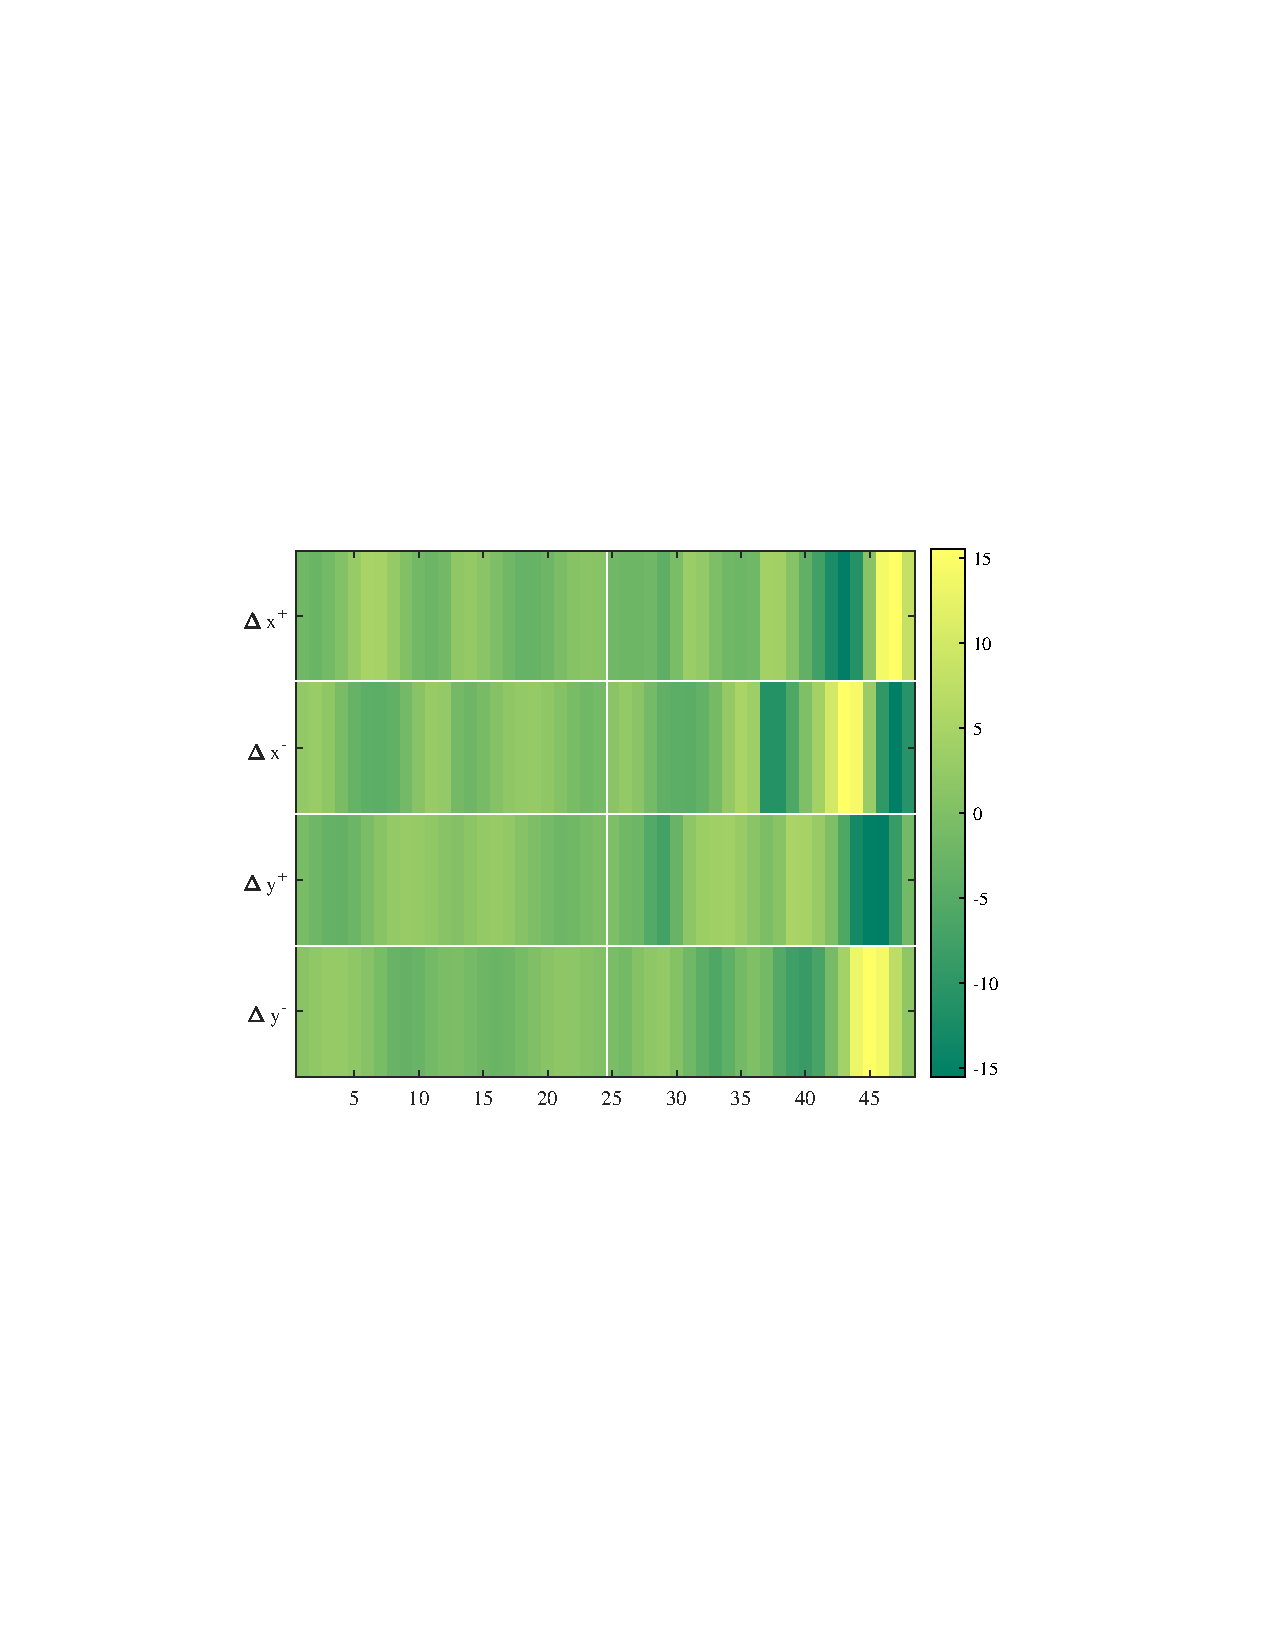
\includegraphics[width=\linewidth]{Figures/Synaptic Weights - BRC.pdf}
        \caption{Synaptic Weights before Reward change}
        \label{fig_3_8}
    \end{minipage}
    \hfill
    \begin{minipage}{0.48\textwidth}
        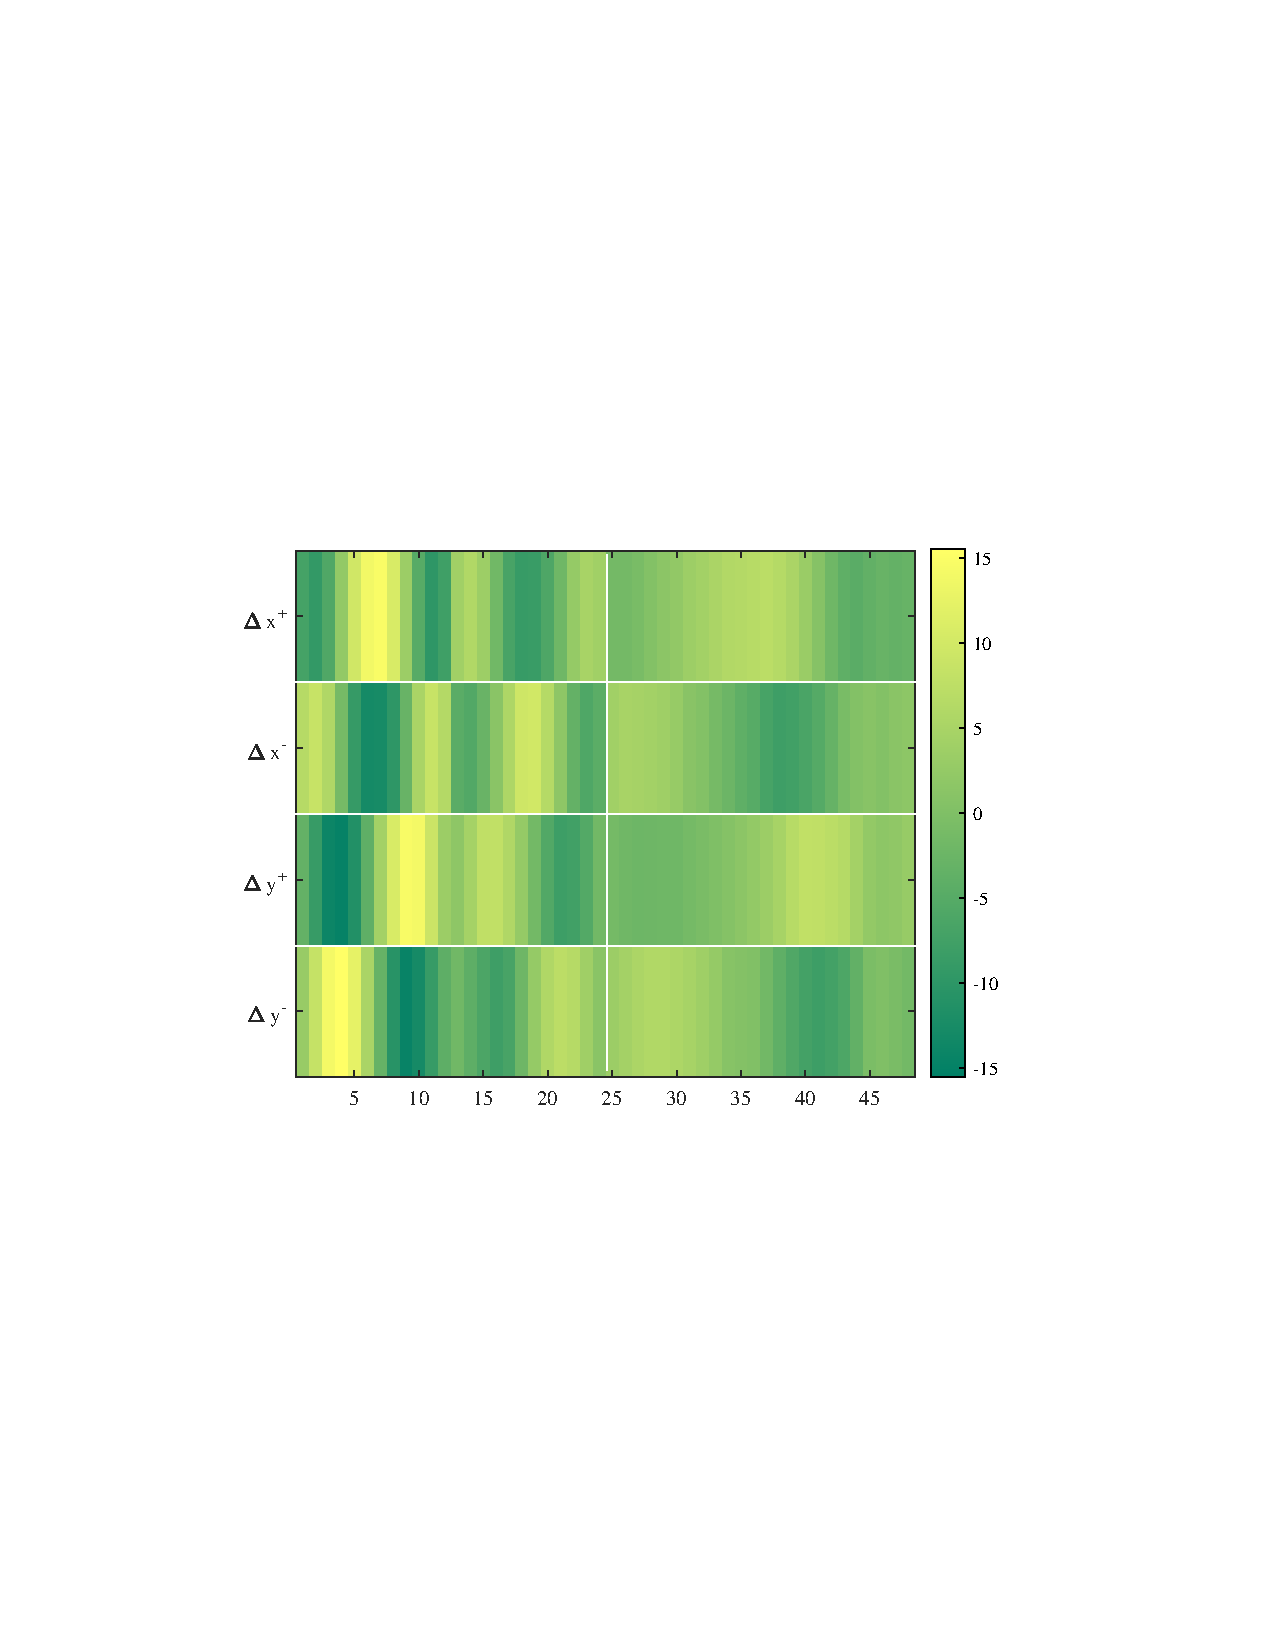
\includegraphics[width=\linewidth]{Figures/Synaptic Weights - ARC.pdf}
        \caption{Synaptic Weights after Reward change}
        \label{fig_3_9}
    \end{minipage}
\end{figure}

\begin{figure}[!h]
    \centering
    \begin{minipage}{0.48\textwidth}
        \includegraphics[width=\linewidth]{Figures/RLST - Weight Increase.pdf}
        \caption{Synaptic weights increase after reward change}
        \label{fig_3_10}
    \end{minipage}
    \hfill
    \begin{minipage}{0.48\textwidth}
        \includegraphics[width=\linewidth]{Figures/RLST - Weight Decrease.pdf}
        \caption{Synaptic weights decrease after reward change}
        \label{fig_3_11}
    \end{minipage}
\end{figure}

According to Figure \ref{fig_3_8}, we can see a gradual change in weights because of the fuzzy nature of the input. Since the reward coefficients for followers and leaders are different, there is a difference in the maximum allowed synaptic weight for them. The proposed method for controlling the unbounded growth of synaptic weights has successfully stabilized the network while maintaining the fuzzy patterns of the synaptic connections.

Figure \ref{fig_3_9} shows the synaptic weights after the reward change. In this case, since the reward coefficients are changed, the \(\eta\) and \(\beta\) values are changed for the represented sub-layers, and the proposed method has helped the \ac{stdp} algorithm to adjust the weights based on the new situation in the environment.

\subsection{Simulation with \ac{fl} and \ac{RCSE}}

In this section, the proposed aggregation algorithm is tested. In this case, the agents only send their models when the Euclidean distance between the current and previously published model or the latest global model reaches a threshold. In the first phase, the simulation was done in 600 seconds, and the agents learned to follow the leader. The threshold for publishing the agents' and server models was 0.0005 and 0.00051, respectively. The reason for choosing the server's threshold a little bit higher than the agents' is that as soon as the first agent sends its model to the server, the Euclidean distance between the current and previously published model by the server reaches 0.0005, and the server distributes the model immediately. Therefore, the serve's threshold is set higher than the agents' threshold so that it waits for the other agents to send their models.

Figure \ref{fig_3-7} shows the distances between agents and the leader before the reward change. According to the figure, the agents converge to the solution faster than the non-\ac{fl} scenario without any error. Figure \ref{fig_3-8} shows the simulation results for the reward change scenario. According to the figure, the proposed aggregation method has improved the learning performance so that the swarm converges to the solution in 6 seconds.

\begin{figure}[H]
    \centering
    \begin{minipage}{0.48\textwidth}
        \includegraphics[width=\linewidth]{Figures/Distances - BRC - DAI.pdf}
        \caption{Distances during the test phase before reward change in the proposed aggregation method.}
        \label{fig_3-7}
    \end{minipage}
    \hfill
    \begin{minipage}{0.48\textwidth}
        \includegraphics[width=\linewidth]{Figures/Distances - ARC - DAI.pdf}
        \caption{Distances during the test phase after reward change in the proposed aggregation method.}
        \label{fig_3-8}
    \end{minipage}
\end{figure}

The norm of the synaptic weights can represent the changes in the synaptic weights due to the change in the environment during the training process, which can be used as an index to adjust the learning process in SNNs. The proposed aggregation method helps SNN models converge into a single model. Agents communicate with the Central Server (leader) during the training process, and Figure \ref{fig:3-10} shows the communication times. The aggregation step time is small at the beginning of the training and increases as the SNN models converge to the final solution. The rate of change of norm of the synaptic weights determines the principle of the aggregation process, which results in small intervals of aggregation when the change rate is high, and larger intervals when it reduces.

\begin{figure}[H]
    \centering
    \begin{minipage}{0.48\textwidth}
        \includegraphics[width=\linewidth]{Figures/Norm.pdf}
        \caption{Frobenius norm of the agents during the learning phase. The reward changes for the Leader after 600 s.}
        \label{fig:3-9}
    \end{minipage}
    \hfill
    \begin{minipage}{0.50\textwidth}
        \includegraphics[width=\linewidth]{Figures/Communication Log.pdf}
        \caption{Communication times for agents and the Central Server (Leader). Red and blue dots show the times that agents and the Central Server have sent their model, respectively.}
        \label{fig:3-10}
    \end{minipage}
\end{figure}


Therefore, the aggregation frequency is very high initially, and it reduces after the change in synaptic weights goes to zero because of the learning rate in (\ref{Eq.WS.1}). Also, after the reward changes and the leader becomes an obstacle after 600 seconds, the Euclidean distance between the converged and current models increases and reaches the threshold. As soon as the first agent sends its model to the server, the aggregation process starts again, and the agents adjust the associated synaptic weight.

\begin{table}[H]
    \centering
    \small
    \caption{Comparative Performance Analysis of the Proposed Aggregation Algorithm+\ac{RCSE}, \ac{RCSE}, and FACL}
    \begingroup
    \renewcommand{\arraystretch}{1.5}
    \begin{tabular}{lccc}
    \hline
                                & \textbf{FL+\ac{RCSE}} & \textbf{\ac{RCSE}} & \textbf{FACL} \\
    \hline
    \textbf{Learning Time - Training Phase (s)}                & 261.92               & 554.71      & 667.26                   \\
    \textbf{Max Error After Convergence - Test Phase (\%)} & 0.71             & 1.95     & 9.85                 \\
    \textbf{Convergence Time - Test Phase (s)}             & 5.81           & 8.94     & 15.82                   \\
    \hline
    \end{tabular}
    \endgroup
    \label{tab:Results analysis}
\end{table}


Table \ref{tab:Results analysis} compares the proposed \ac{fl} algorithm with the non-FL approach and FACL algorithm. The comparison focuses on three critical metrics: learning time, maximum error after convergence, and convergence time. The proposed \ac{fl} algorithm demonstrates significant improvements in terms of efficiency and accuracy, as evidenced by its considerably shorter learning and convergence times and a notable reduction in error after convergence.

\section{Conclusion}

In this chapter, we presented a comprehensive approach addressing the challenges of uncontrolled growth in synaptic weights and the limited responsiveness of \ac{stdp} to real-time changes within \ac{snn}s. Our proposed solution integrates the \ac{RCSE} method with a dynamic aggregation interval in \ac{fl}, significantly reducing learning time and improving performance.
The R-CSE method introduces a novel mechanism to manage the unbounded growth of synaptic weights by dynamically adjusting the decay rate through the SoftPlus function. This adjustment is sensitive to the learning stages and rewards changes, ensuring that synaptic weight adjustments remain responsive over time. By addressing the challenge of synaptic weight saturation, the \ac{RCSE} method facilitates a balanced approach to weight adjustment, preventing network saturation and promoting continuous learning adaptability.

We introduce a novel approach that uses \ac{fl} in SNN and employs the Frobenius norm to adjust weighted aggregation in \ac{fl}. Additionally, we include weight decay proportional to the time elapsed since an agent's last model publication. This improves the efficiency and responsiveness of the learning process. 
Our model's dynamic nature of the model aggregation time adjusts based on the Euclidean norm. This metric measures the distance between the weight matrices of the agents and the server, determining reduced intervals for model publication. Our results show that the proposed aggregation method significantly accelerates agents' learning and performs better than non-\ac{fl} and \ac{facl} cases.

Moreover, the dynamic aggregation interval effectively reduces communication overhead between the agents and the central server, particularly after model convergence. This reduction is critical in scenarios where communication bandwidth is limited or costly. 
Our findings suggest that integrating \ac{stdp} with \ac{fl}, supported by our dynamic aggregation approach, provides a robust framework for advancing multi-agent reinforcement learning systems.